% !TEX root = ../paper.tex
\section{Design}
\subsection{Design Summary}
Lean 4 is a good target for our translation as well as a suitable language to implement our translation in because of the fact that Lean 4 is mostly implemented in itself. As users, we are able to utilize and emit the same data structures used in Lean's own implementation to extend the functionality of Lean \cite{moura2021lean}. These metaprogramming capabilities of Lean make our work implementing a Forge module in Lean much easier. 

The Lean 4 compilation process is structured as follows:
\begin{figure}[h!]
\centering
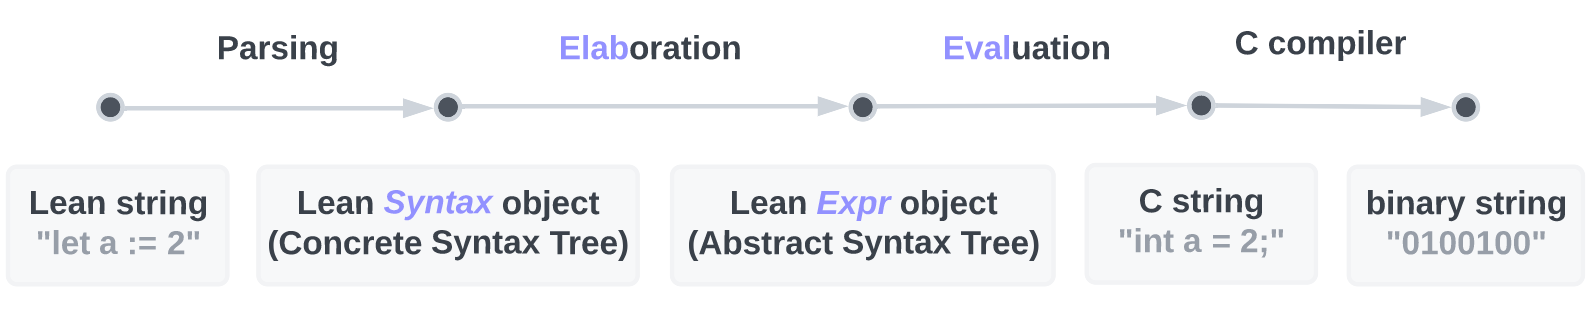
\includegraphics[width=0.8\textwidth]{images/lean-compiler.png}
\caption{A diagram from \cite{metaprogramming} summarizing the Lean 4 compilation process.}
\end{figure}

Specifically, the parsing and elaboration steps are designed to be highly customizable and are provided as a `first-class' feature of Lean 4. We approach the problem of translating Forge into Lean as a task of adding new language features to Lean itself. We define new Lean syntax objects that correspond to a concrete syntax tree of Forge and implement a parser for Forge (see \cref{sec:parsing}), and then implement a custom elaboration function for our Forge syntax to translate it into native Lean expressions (see \cref{sec:elaboration}). 

As a result, there as little additional overhead as possible when translating a Forge specification in Lean. After users have imported our module, all Forge expressions \emph{are} valid Lean expressions and the two languages can be used interchangeably\footnote{We are very fortunate that there are no conflicts between Forge and Lean syntax that would hinder this.}.\todo{complete?}

\subsection{Syntax, Parsing, and the Forge AST}\label{sec:parsing}
In the case of parsing, by defining the Forge grammar in the same specification format that Lean defines its syntax in, we can rely on Lean's parser to parse Forge source code for us.

The benefits of this are two-sided:
\begin{enumerate}
  \item We are provided Lean \texttt{Syntax} objects at the end of this process, the same type that parsing a Lean program would produce. This enables us to treat our Forge implementation as implementation of additional Lean language features, and we can also harness Lean metaprogramming libraries along the way. This is to say, we are implementing Forge in Lean the \emph{same way} Lean is implemented in Lean, which greatly reduces our burden for additional implementation overhead.
  \item By defining Forge `blocks' as a Lean \texttt{command}---which is the top-level syntax category\footnote{For example, a definition ``\texttt{def x: Int := 0}'' is a Lean command.}---users of the tool can insert raw Forge, without any annotations that this is an ``extension language'', into Lean. With the addition of an import statement, every Forge program \emph{is} a valid Lean program.
\end{enumerate}

Lean allows us to create \emph{syntax categories} for each term\todo{variable?} in our grammar. At the top-level, we have defined \texttt{f\_sig} (Sigs), \texttt{f\_pred} (Predicates), \texttt{f\_fun} (Functions). Terms are either \texttt{f\_fmla} for formulas (evaluate to True or False) or \texttt{f\_expr} for expressions (evaluate to a set, relation, int).

For example, the grammar\footnote{Where $,+$ and $,*$ denote one/zero or more comma-separated occurrences respectively. $+$ and $*$ denote one/zero or more repetitions.} of Forge arguments and predicates is:

\vspace{1em}\begin{center}
\begin{minipage}{0.8\textwidth}
\setlength{\grammarindent}{6em}
\begin{grammar}
<arg> ::= <ident>,+ `:' <expr>

<args> ::= <arg>,*

<pred> ::= `pred' <ident> [`[' <args> `]'] `{' <fmla>* `}'
\end{grammar}
\end{minipage}
\end{center}

Which we can translate into a corresponding syntax definition in Lean:
\begin{leanimpl}
declare_syntax_cat f_arg
syntax ident,+ ":" f_expr : f_arg

declare_syntax_cat f_args
syntax f_arg,* : f_args

declare_syntax_cat f_pred
syntax "pred" ident ("[" f_args "]")? "{" f_fmla* "}" : f_pred
\end{leanimpl}

Following this blueprint, we are able to translate the entirety of the grammar of Forge\footnote{At least, a useful subset of the Forge language we care about. This is based off the grammar of Alloy \cite{jackson2012software,jackson2019alloy,ngpdbccdlrrvwwk-oopsla-2024}.} into Lean syntax definitions.

What remains to be done is to convert syntax, almost one-to-one, into an AST for Forge, and then \emph{elaborate} (see \cref{sec:elaboration}) our AST into Lean expressions and declarations.

\begin{leanimpl}
structure Predicate where
  name : Symbol
  name_tok : Syntax
  args : List (Symbol × Expression) -- (name, type) pairs
  body : Formula -- with args bound
  deriving Repr, Inhabited   
\end{leanimpl}

\subsection{Elaboration}\label{sec:elaboration}
\todo{Complete}

\subsection{The Forge Model in Lean}\label{sec:forge-model}
\todo{Complete}

% Table of things in Forge and their translation in Lean
